%%%%%%%%%%%%%%%%%%%%%%%%%%%%%%%%%%%%%%%%%
% Press Release
% LaTeX Template
% Version 1.0 (2/6/13)
%
% License:
% CC BY-NC-SA 3.0 (http://creativecommons.org/licenses/by-nc-sa/3.0/)
%
%%%%%%%%%%%%%%%%%%%%%%%%%%%%%%%%%%%%%%%%%

%----------------------------------------------------------------------------------------
%	PACKAGES AND OTHER DOCUMENT CONFIGURATIONS
%----------------------------------------------------------------------------------------

\documentclass[11pt,pressrelease]{newlfm} % Font size

\usepackage{charter} % Use the Charter font for the document text
\usepackage{hyperref}


\PhrPhone{Phone} % Customize the "Telephone" text
\PhrEmail{Email} % Customize the "E-mail" text
%\PhrContact{Contact} % Uncomment this line to change the 'Contact:' text

%----------------------------------------------------------------------------------------
%	PRESS RELEASE INFORMATION
%----------------------------------------------------------------------------------------

\makeletterhead{Uiuc}{\Cheader{\vspace{16pt}
\includegraphics[width=0.3\linewidth]{TSF_Logo_NB.jpg}}} % Include a company logo, if you don't use one you will need to uncomment line 6 in the prsrls.tex file
\lthUiuc % Print the company/institution logo

\release{For Immediate Release to Tartan Student Fund} % When the press release may be used

\namefrom{David Hiles, Head of Allocation} % Name

\phonefrom{732-796-8352} % Phone number

\emailfrom{dhiles@cmu.edu} % Email address

\headline{Portfolio Updates} % Headline for the press release

\newcommand{\subtitle}{This is a subtitle to the headline giving more information about the headline.}  % Subtitle for the press release, if you don't want one just remove the subtitle text leaving the rest of the command

\byline{\textbf{Carnegie Mellon University, -- \today ~--} \$FITB, Healthcare \& Macro Themes} % A summary line for the press release

%----------------------------------------------------------------------------------------

\begin{document}
\begin{newlfm}

%----------------------------------------------------------------------------------------
%	PRESS RELEASE CONTENT
%----------------------------------------------------------------------------------------

\vspace{-.25 in} 			%.25  is normal
\begin{singlespace} 		% Uncomment for single line spacing

\begin{enumerate}
\item \textbf{Fifth Thirds Bank } \par
We will be taking an average sized position in \$FITB. RRS thought this was one of the strongest pitches this semester. We are very interested to see how political catalysts will effect this industry. We saw a strong price appreciation after the election results. While RRS does not hold political views, we are focused on  Trump's proposed deregulation of the banking industries and a hawkish Fed stance. We were also impressed with the balance sheet composition and believe that this bank is well positioned in its space. 

\item \textbf{Healthcare} \par
As reported in our last summary, the healthcare group has been our lagging portfolio group this year. Many of our companies in this portfolio had implicit risks we did not understand when taking a position: pipeline and regulatory being the largest. We will be considering underweight the healthcare group (vs the S\&P 500 weighting) as the semester comes to a close. Closer monitoring of our positions, including qualitative business changes, will be monitored more carefully in the future. 

\item \textbf{Theme-in-a-Chart} \par
Again, we want to reiterate our lack of political bias in our analysis. However, new political catalysts could pose an interesting thematic change in equity markets. Months before the election, we saw an interesting pattern: rising growth without higher bond yields. We have seen equity valuations move higher with steady growers AND bond proxies (safe strong dividends) outperforming.  However, post election, we have seen a trend pointing to a reflation scenario. In this new regime, we can rising growth (a relatively novel idea in the past 3 years) but with higher bond yields moving up; this is supported by the Fed as well. In this theme, equities should move higher (all time highs in sight) BUT ONLY as earnings improve. However, we see a countering effect: as yields rise, we will see an increase in the borrowing costs of businesses, limiting valuations. This will put more emphasis on earings and earnings growth. As we have seen already post-election, cyclicals and financials should outperform.

\newpage
As we can see by this chart, the market has begun to anticipate a rise in inflation; this chart uses 10 year and 5 year TIPS (Treasury Inflation Protected Securities) to back out an inflation expectation.
\begin{center}
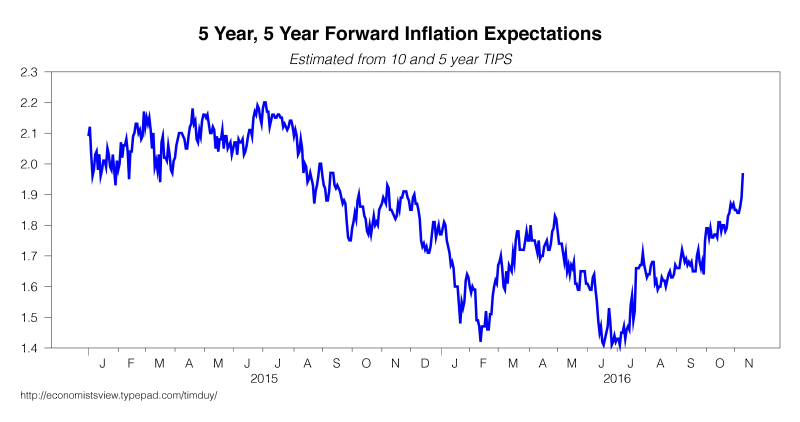
\includegraphics[width=.8\textwidth]{5_year_inflation.jpg}
\end{center}

Following the first two bullet points, we think this theme of high inflation could be a beneficial environment for Fifth Thirds Bank as well as the rest of the financials group. Healthcare tends to preform better in this environment, however this has yet to be seen. We will now be rotating our focus to the TMT group as higher inflation causes costs to rise and reduces the spending power of consumers, which could be worrisome for the technology sector.

%\item \textbf{Dave's Trade}: Company has considerably outperformed YTD, gun sales are record high in this election year and and I see no reason to see this trend slow.

\end{enumerate}
\par

We are looking forward to the concluding meeting including the discussions about our allocations including a plan during the winter dead period. \par Lastly, I hope you all have a wonderful Thanksgiving.

\vspace{2.5in}
Thank you, \par
Research, Risk and Strategy


\end{singlespace} % Uncomment for single line spacing


%----------------------------------------------------------------------------------------

\end{newlfm}
\end{document}